\documentclass[12pt]{article}
\usepackage{natbib}
\usepackage{natbib,letltxmacro}
 \usepackage{float}
\usepackage{lineno}
\usepackage{subfigure}
\usepackage[english]{babel}
\usepackage{parskip}
\usepackage{tocloft}
% Set page size and margins
% Replace `letterpaper' with `a4paper' for UK/EU standard size
\usepackage[a4paper,top=2cm,bottom=2cm,left=2.5cm,right=2.5cm,marginparwidth=1.75cm]{geometry}

% Useful packages
\usepackage{amsmath}
\usepackage{graphicx}
\usepackage[colorlinks=true, allcolors=blue]{hyperref}

\title{Predicting the Identity and Abundance of Globally-Important Tyrosinase Genes in Bacteria Based on Metagenomics and Machine Learning}
\author{Mingji Zhang (mz522@imperial.ac.uk)\\\\
Supervised by :\\
Samraat Pawer ( Imperial College London)}
\date{Apr,2023}
\footnotetext[2]{CMEECoursework,Department of Life Sciences, Imperial College of Science, Technology and Medicine}

\begin{document}

\maketitle
\newpage
\tableofcontents
\newpage
\pagenumbering{arabic} 
\setcounter{page}{1} 
\maketitle

\newgeometry{margin=2cm}
\begin{abstract}

Microbial communities play a pivotal role in ecosystem functions, including carbon cycling and climate regulation. Targeting the Tyrosine Recombinase (TYR) gene, a key enzyme in aromatic compound metabolism, I delves into the identification of potential bacterial hosts within different aqueous environments. Leveraging metagenomic data and employing advanced machine learning techniques, a comprehensive analysis unveils intricate relationships between TYR gene abundance and microbial hosts across diverse ecosystems. My study's innovative approach encompasses multivariate linear regression and correlation network modeling, shedding light on the ecological and functional significance of TYR genes in distinct environments. Results highlight correlations between TYR gene abundance and specific genera such as Gemmiger, Escherichia, Collisella, Streptococcus, Akkermansia, Bifidobacterium, Faecalibacterium, and the yet-to-be-identified \text{k\_\_Bacteria|p\_\_Firmicutes|c\_\_CFGB10477|o\_\_OFGB10477|f\_\_FGB10477|}\\
\text{g\_\_GGB9345} bacteria. This suggests that these genera might play a crucial role in aromatic compound metabolism. The Alpha and Beta diversity analyses further uncover compelling trends: certain environments display a prevalence of these TYR gene-associated genera, potentially indicating their ecological significance. These findings underscore the potential of machine learning for predicting TYR gene abundance and host organisms, offering a promising alternative to costly molecular diagnostics.  Although limitations exist, including dataset representation and unaccounted variables, my study still advances the understanding of TYR gene dynamics and its ecological implications in different environments, contributing to the fields of environmental microbiology and carbon cycling research.\\\\

\textbf{Keywords:} Metagenomics, Tyrosinase genes, Microbial communities, Machine Learning, Abundance prediction, Environmental diversity
\end{abstract}
\restoregeometry


\newpage
\section{Introduction}

Global warming, as a major challenge facing the world today, has aroused widespread concern and worry \citep{helbling2023global}. Its impact not only covers the climate system, but also involves a wide range of fields such as socio-economics and ecology \citep{sodangi2011climate,grace2004understanding,falkowski2000global,wani2023multi} Against this urgent background, the role of the global carbon cycle has become more and more important, as it carries a huge potential for curbing global warming \citep{falkowski2000global}. The global carbon cycle is a complex ecological process involving the exchange and cycling of carbon between the atmosphere, land and ocean \citep{grace2004understanding,falkowski2000global}. The biosphere converts carbon dioxide into organic matter through photosynthesis, storing it in plants, soil and oceans \citep{wani2023multi}. This organic matter gradually releases carbon dioxide during decomposition and biological processes, creating a balanced carbon cycling system \citep{wani2023multi}.     The soil carbon pool is one of the five important carbon pools of the Earth, absorbing and storing large amounts of carbon dioxide and slowing down the accumulation of greenhouse gases in the atmosphere through its dynamic interaction with the biosphere carbon pool \citep{wani2023multi}. Plants in ecosystems absorb large amounts of carbon dioxide through photosynthesis and fix it in their organisms, thus reducing the release of greenhouse gases \citep{falkowski2000global}. At the same time, microorganisms in the ecosystem are also involved in carbon decomposition and transformation, influencing the rate and direction of the carbon cycle \citep{hawkins2023mycorrhizal,de2020microbial}. Soil respiration is the main pathway by which carbon dioxide fixed by land plants is returned to the atmosphere\citep{schlesinger2000soil}. Therefore, maintaining the integrity and diversity of ecosystems and protecting vegetation and soils are essential for the stabilization of the global carbon cycle \citep{wani2023multi}.\\\\
Tyrosinases (TYRs) are important phenolic oxidases that are widely involved in the global carbon cycle and play a key role, especially in some ecosystems that exhibit high phenolic compounds \citep{panis2022novel,panis2021expression}. TYRs are found in bacteria and eukaryotes and catalyze the oxidation of tyrosine and other phenolic compounds \citep{panis2022novel,hassan2023tyrosinase,panis2021expression}. TYRs are involved in the degradation and transformation of organic carbon in the environment, facilitating the decomposition and conversion of organic matter into more stable forms, thereby influencing carbon storage and release processes \citep{de2020microbial}. At the same time TYRs catalyse oxidation reactions involving the conversion of phenolic compounds, which play a crucial role in the decomposition and humification of organic matter \citep{de2020microbial}. Historically, persistent waterlogging has limited the activities of TYRs \citep{panis2021expression}. Peatlands store 30\% of global soil carbon, and prolonged summer droughts caused by global warming have facilitated the release of carbon stored as organic compounds from peatland carbon pools by TYRs \citep{panis2021expression}. Understanding the role of TYRs is therefore critical to assessing the impact of carbon dioxide in the global carbon cycle \citep{panis2021expression}.\\\\
However, although the role of TYRs in ecosystems has been recognized to some extent, there is still a knowledge gap in the identification of host environments as well as TYR-positive genera \citep{panis2022novel}. With the continuous development of advanced molecular biology and genome sequencing technologies, second-generation gene sequencing techniques provide for the search for potential TYR-positive genera \citep{slatko2018overview,metzker2010sequencing}. Metagenomic technology provides excellent conditions and opportunities in identifying hosts of specific genes in the environment \citep{wooley2010primer,sleator2008metagenomics}. This technology breaks through the limitations of traditional genetic studies and is no longer limited to studying the genome of a single organism, but is able to simultaneously analyze microbial populations throughout an ecosystem \citep{metzker2010sequencing,wooley2010primer,sleator2008metagenomics}. This provides new possibilities and depth for revealing the hosts of specific genes in the environment.In metagenomic studies, by collecting environmental samples and extracting the microbial DNA from them, the genetic information of all the microbial communities present in this environment can be obtained \citep{wooley2010primer}. Subsequently, a large amount of DNA sequence data is acquired through high-throughput sequencing techniques \citep{daniel2005metagenomics}. These data contain gene sequences from a wide range of microorganisms, which may also cover target genes \citep{daniel2005metagenomics}. Subsequently, through a process of fine-grained data analysis and metagenome assembly, these DNA sequences can be spliced and annotated to determine their possible functions and origins \citep{daniel2005metagenomics,sleator2008metagenomics}. This makes it possible to identify hosts of specific genes in the environment. By comparing databases of known genes, it is possible to determine which groups of microorganisms carry the target genes and thus find their potential hosts \citep{metzker2010sequencing}.\\\\
However, traditional methods for identifying gene-host associations often prove time-consuming and are constrained by prior knowledge of gene functionality \citep{moradigaravand2018prediction,sun2021predicting}. In order to overcome these challenges, recent advancements in machine learning technology have demonstrated the capability to predict specific bacterial hosts of genes even in the absence of prior mechanistic insights \citep{sun2021predicting}. Notably, a study focused on antibiotic resistance genes has indicated that machine learning models can accurately predict resistance patterns solely based on genomic and epidemiological data, even without detailed understanding of underlying biological mechanisms \citep{moradigaravand2018prediction}. Machine learning techniques offer an alternative approach for addressing the link between bacterial species and the TYR gene. Multivariate linear regression modeling is a machine learning algorithm that can predict the abundance of TYR genes based on the analysis of bacterial community abundance data obtained from metagenomic studies \citep{eberly2007multiple}. By modeling multivariate linear regression, potential TYR hosts in the environment can be identified and bacterial species enriched for TYR genes can be identified \citep{eberly2007multiple}.\\\\
The main goal of my research is to bridge the existing knowledge gap in identifying TYR-positive genera in different aqueous environments by applying a robust machine learning framework. I used multiple linear regression analysis to train and model, and I utilized 530 publicly available metagenomic datasets to obtain data on bacterial community abundance and relative gene abundance for the TYR gene. Calculated abundances were then meticulously validated on a comprehensive test dataset, a critical step in evaluating their predictive performance. My study predicted the abundance of TYR genes by employing multiple linear regression fitting and discriminated between bacterial species enriched in TYR genes, which indicate potential TYR hosts. In addition, the inclusion of bacterial taxonomic data in the multiple linear regression analysis helped to accurately predict TYR gene abundance in different sample environments. Predictions were performed based on two taxonomic levels, Family and Genus. To better highlight the great potential of utilizing machine learning techniques to effectively identify potential bacterial hosts responsible for TYR activities in the environment and to reveal the complex dynamics and importance of TYR in global carbon cycle and environmental processes by attempting to explore the intricate ecological associations between the TYR genes and their microbial hosts, I specifically investigated three questions: (1) How well can machine learning techniques be utilized to predict the abundance and TYR-positive genera in host environments? (2) What characterizes the diversity of microbial hosts carrying the TYR gene in different environments? (3) What significant correlations exist between the gene abundance of the TYR gene in different environments and specific bacterial genera?\\\\


\section{Materials and Methods}

\subsection{Bioinformatics analysis}

A total of 530 sample sequences were randomly selected from the National Council for Biotechnology(NCBI) database, encompassing four primary sequencing environments, namely fecal, urban river, sewage, and large river, as well as two special sequencing environments, glacier lacustrine, and groundwater. The selection aimed to include as many bacterial species as possible, ensuring a comprehensive representation of the diverse microbial communities. Detailed information about all the sample sequence numbers can be found in Appendix Table S1.The flowchart of the entire project is shown in Figure 1.
\begin{figure}[H]
    \centering
    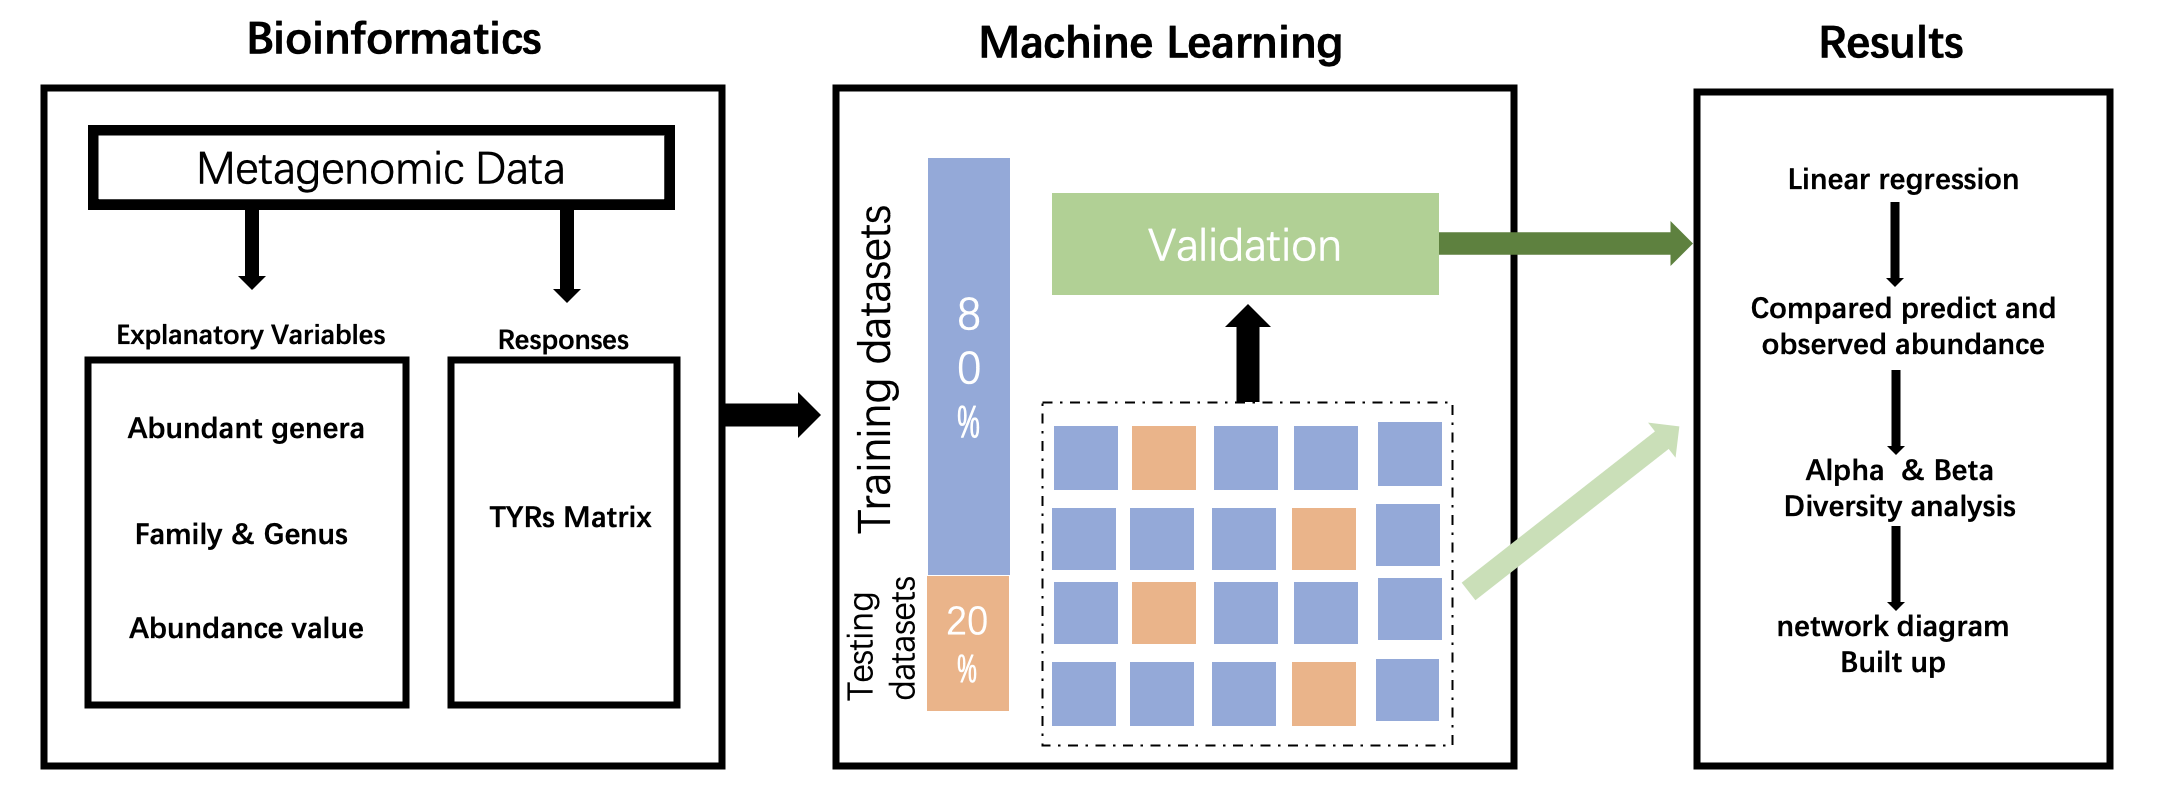
\includegraphics[width=1\linewidth]{pic/flowwork.png} 
    \caption{\small\bfseries Flowchart of the project including three periods.}
\end{figure}

Prior to analysis, all samples underwent meticulous pre-processing using Metagenomic Phylogenetic Analysis (MetaPhlan) 4.0 \citep{segata2012metagenomic}. This preprocessing involved the trimming of macrogenomic sequence reads obtained from public databases, as well as the elimination of low-quality reads and splice sequences \citep{segata2012metagenomic}. The trimmed reads were then employed for strain extraction, facilitating the construction of the relative abundance matrix of the bacterial colonies.\\\\
Using a query term "tyrosinase," I employed a search of the NCBI database to target the TYR gene sequences, leading to the identification of 74,283 entries (as of May 2023). Subsequently, a reference short sequence library was curated, encompassing all the short sequence entries. The open-source programme DIAMOND (Dual Index Alignment of Next Generation Sequencing Data) was used to carry out comparisons between samples and reference libraries \citep{buchfink2015fast}. Whenever a sequence in a sample displayed a precise overlap with a sequence in the database, extending over a span of 25 or more amino acids, it was considered as a TYR sequence \citep{kristiansson2011pyrosequencing}. In addition, relative abundance values were uniformly normalised to parts per million (ppm) units for ease of comparison and analysis \citep{yang2013exploring}. This normalisation standardises abundance measurements across samples, allowing for meaningful comparisons of the presence and abundance of tyrosinase genes in different sequencing environments \citep{yang2013exploring}.


\subsection{Development, validation and application of multiple linear regression model}

A multivariate linear regression model was developed using the S2 relative abundance matrix and the S3 gene abundance matrix, which was obtained by rigorous data pre-processing as described in section 2.1. The multiple linear regression model is represented as follows \citep{eberly2007multiple}:
\[
y = \beta_0 + \beta_1 x_1 + \beta_2 x_2 + \ldots + \beta_p x_p + \varepsilon
\]

where:
\begin{align*}
y & : \text{The dependent variable (the target variable to be predicted).} \\
x_1, x_2, \ldots, x_p & : \text{The independent variables (features or predictors).} \\
\beta_0 & : \text{The intercept term, representing the predicted value of } y \text{ when all } \\
& \quad \text{independent variables(\(x_1, x_2, \ldots, x_p\)) are set to zero.} \\
\beta_1, \beta_2, \ldots, \beta_p & : \text{The coefficients, indicating the impact of each independent variable on } \\
& \quad \text{the predicted value of the dependent variable \(y\).} \\
\varepsilon & : \text{The error term (residual), accounting for the discrepancy between the} \\
& \quad \text{predicted and actual values of the dependent variable \(y\). } \\
& \quad \text{It captures the unexplained variation in the predictions.}
\end{align*}

The goal of multiple linear regression is to estimate the coefficients (\(\beta_0, \beta_1, \ldots, \beta_p\)) that minimize the sum of squared errors, resulting in the best-fitted linear model for predicting \(y\) based on the given set of independent variables (\(x_1, x_2, \ldots, x_p\)).

When multivariable linear regression is employed for predicting the abundance of the TYR gene within a sample, the equation can be expressed as follows::\\\\
\begin{align*}
   \text{The prediction abundence (} A \text{)}&= \sum_{s} S_i \cdot A_s \\
\end{align*}
where:
\begin{align*}
    A & : \text{ represents the total TYR gene's abundance of the sample,} \\
    S_i & : \text{ represents the relative bacterial abundance of each species in the sample,} \\
    A_s & : \text{ represents the TYR abundance of each species.}
\end{align*}

The analysis was performed using the Scikit-learn(sklearn) package in R, which incorporates some basic steps such as data normalisation, missing value handling, data partitioning, preprocessing, model adjustment and variable significance assessment \citep{pedregosa2011scikit,bisong2019introduction,kramer2016scikit}.\\\\
Linear regression analyses were conducted to determine whether there was a statistically significant relationship between the sample variables \citep{maulud2020review}. This analytical procedure is crucial as it ensures the robustness and interpretability of the predictive model \citep{bisong2019introduction}. By employing linear regression, I aimed to explore potential dependencies and correlations between the variables, thereby laying a solid foundation for subsequent modelling and prediction tasks. The rigour of the linear regression analysis contributes to the reliability and validity of the findings, leading to meaningful interpretations and in-depth analyses of the potential relationships between the variables under investigation. In addition, 95\% confidence intervals were incorporated to account for sample uncertainty and to provide a measure of confidence in the correlation \citep{ci1987confidence}. This correlation validation process is essential to determine the statistical significance of TYR gene abundance predictions and to gain insight into the relationships between other genes or environmental factors and TYR gene expression, thereby enhancing our understanding of TYR gene function.\\\\
The development of the model involved several steps. Firstly, I randomly divided the samples into an 80\% training subset and a 20\% validation subset using the sklearn package to ensure the balance of samples in both subsets \citep{kramer2016scikit}. Next, we utilized the training function from the sklearn package to generate multiple linear regression models separately based on the Family and Genus dimensions \citep{bisong2019introduction}. This approach allowed us to make predictions at both the Family and Genus taxonomic levels.\\\\
Predictions based on the Family level exhibit a higher degree of aggregation, encompassing a wider range of different bacterial species, thus capturing common features across different bacterial genera. This broad aggregation aids in identifying overall trends and patterns in the data, especially when the sample size is small or the number of bacterial species is large, resulting in more reliable results. Furthermore, due to the relatively high Family classification, the prediction results are more generalized, facilitating an understanding of the overall relevance of the bacterial community to TYR genes.\\\\
On the other hand, predictions based on the Genus level are more refined and detailed, enabling a more accurate differentiation of different bacterial genera. This fine-grained prediction approach is instrumental in capturing subtle differences and ecological associations between different bacterial genera. In cases of larger sample sizes or fewer bacterial species, Genus-level predictions provide more precise information, unveiling specific relationships between bacterial genera and TYR genes.\\\\
To ensure the model's reliability and generalizability, I recorded the intercepts and coefficients for each fitted model on the validation set. Subsequently, we ranked all sample regression coefficients and grouped them into high and low correlation categories based on the absolute value of the coefficients. Random cross-validation was conducted to ensure predictive accuracy.\\\\
In addition, as an integral part of the model evaluation process, I compared the validation set gene abundance obtained through model fitting to the observed gene abundance. This rigorous evaluation process allows for a quantitative comparison between the predicted gene abundance and the actual gene abundance in the validation set, thereby determining the accuracy and reliability of the model predictions.\\\\

\subsection{Statistical analysis and data visualization}

In order to visualise the predictions, the Matplotlib package \citep{barrett2005matplotlib} for python was used to present the results of the linear regression. The scatterplot visualises the correlation between the variables. A direct comparison between predicted and actual values is shown in a line graph. The line graph description provides a visual assessment of the accuracy of the predictions. Sample's phylum level histograms were plotted by Origin software \citep{edwards2002origin} and ggplot \citep{wickham2006introduction} to show the number or abundance of bacterial species under different phylums. The distribution of the major phyla of bacteria can be visualised. The Alpha diversity and Beta diversity analysis plots used to assess the diversity of bacterial species and differences in species composition within the samples were plotted by ggplot in R.The Alpha diversity was calculated using Shannon Diversity formula. The formula was calculated as follow \citep{nolan2006beachcomber}:
\begin{align*}
\text{Shannon Diversity Index (} H' \text{)} & = - \sum_{i=1}^{S} p_i \cdot \ln(p_i) \\
\end{align*}
where:
\begin{align*}
H' & : \text{represents the Shannon diversity index,} \\
S & : \text{represents the total number of species in the community,} \\
p_i & : \text{represents the proportion or relative abundance of the i-th species}\\
& \quad \text{in the community.}
\end{align*}
The Beta diversity was calculated using the Bray-Curtis algorithm. The formula was calculated as follows \citep{beals1984bray}: 
\begin{align*}
\text{Bray-Curtis distance (BC)} & = \frac{\sum{|a_i - b_i|}}{\sum{(a_i + b_i)}} \\
\end{align*}
where:
\begin{align*}
a_i & : \text{represents the abundance or frequency of the i-th species in sample A}, \\
b_i & : \text{represents the abundance or frequency of the i-th species in sample B}.
\end{align*}
Key strains derived from differential expression calculations and Pearson correlation calculations were performed with TYR genes. The following formula was used \citep{cohen2009pearson}: 
 \begin{align*}
\text{Pearson correlation coefficient (r)} & = \frac{\sum{(X_i - \bar{X})(Y_i - \bar{Y})}}{\sqrt{\sum{(X_i - \bar{X})^2}\sum{(Y_i - \bar{Y})^2}}} \\
\end{align*}
where:
\begin{align*}
X_i & : \text{represents the i-th observation of variable X}, \\
Y_i & : \text{represents the i-th observation of variable Y}, \\
\bar{X} & : \text{represents the mean of all observations of variable X}, \\
\bar{Y} & : \text{represents the mean of all observations of variable Y}.
\end{align*}
To determine differentially expressed genes, a significance test is performed in the differential expression analysis to assess whether the observed differences are due to random factors. The p-value is obtained through the t-test. 
The calculation formula for the p-value is as follows \citep{ho2019moving}:

\[
t = \frac{\bar{D}}{s_D / \sqrt{n}}
\]

where:
\begin{align*}
t & : \text{t-statistic}, \\
\bar{D} & : \text{mean of the differences between paired samples}, \\
s_D & : \text{standard deviation of the differences between paired samples}, \\
n & : \text{number of paired samples}.
\end{align*}

A smaller p-value indicates that the observed differences are likely to be real rather than due to chance variation \citep{ho2019moving}. The significance level is set to 0.05, meaning that when the p-value is less than 0.05, the differences are considered significant \citep{kim2015t}. If the p-value is smaller than the predefined significance level, the null hypothesis can be rejected, indicating that the differences are significant \citep{ho2019moving}.

The Log2 Fold Change (Log2FC) is a measure used to quantify the degree of differential expression \citep{erhard2018estimating}. It represents the fold change in gene expression levels between two groups of samples. The formula for Log2FC was calculated as follows \citep{erhard2018estimating}:
\begin{align*}
\text{Log2FC} & = \log_2 \left( \frac{\text{Expression in Treatment Group}}{\text{Expression in Control Group}} \right) \\
\end{align*}
where:
\begin{align*}
\text{Log2FC} & : \text{Log2 Fold Change value}, \\
\log_2 & : \text{logarithm base 2}, \\
\frac{\text{Expression in Treatment Group}}{\text{Expression in Control Group}} & : \text{ratio of gene expression in the treatment} \\
& \quad \text{group to gene expression in the control group}.
\end{align*}



A positive Log2FC indicates that the gene's expression level is higher in the first group of samples compared to the second group, while a negative Log2FC indicates that the gene's expression level is higher in the second group.The calculation was completed to get the correlation coefficient between them. The strains that were significantly correlated with the TYR gene were screened out and these strains were constructed into an association network diagram using Gephi software \citep{bastian2009gephi}. The association network diagram visualises the strains significantly associated with the TYR gene and the association between them. This helps to understand the interactions between TYR genes and specific strains, and may reveal the potential role of TYR genes in regulating the abundance or function of these strains. In addition, the association network diagrams may also provide clues for further functional analyses and biological interpretations to help us better understand the associative relationships between TYR genes and gut microbial communities.\\\\

\section{Result}
A total of 530 metagenomic datasets were selected based on the defined criteria as outlined in Table S1. In May 2023, a comprehensive collection of 530 metagenomic datasets was procured from the NCBI database in the form of FASTQ files. Within these datasets, 125 datasets corresponded to fecal environments, 168 datasets to sewage environments, 176 datasets to urban river environments, 16 datasets to glacier lake environments, 9 datasets to groundwater environments, and 36 datasets to large river environments. The DNA read counts for individual samples spanned a range from 515,744 to 111,343,794, with a mean value of 26,972,889. Across this diverse compilation of datasets, taxonomic classification encompassed 10 phyla, 45 classes, 51 orders, 66 families, 153 genera, and 11,709 species.\\\\
From Figure 2, it can be observed that the TYR gene-containing microbial communities exhibit a diverse array of microbial phyla, and significant variations in relative abundances among these phyla are evident. Among the identified phyla, several show relatively higher relative abundances and count values, indicating their prominent presence and richness in the samples. Specifically, Proteobacteria, Bacteroidetes, and Firmicutes emerge as the most abundant phyla, with relative abundances of 530, 523, and 502, respectively, and correspondingly high count values, further emphasizing their significance within the TYR gene-containing microbial communities. These phyla are known to be widely distributed in soil and other sample sources, suggesting their potential roles in various environmental contexts.\\\\
Moreover, Figure 2 highlights certain microbial phyla that exhibit higher relative abundances and count values in specific samples, such as Actinobacteria, Synergistetes, and Tenericutes. This suggests that these phyla might be sensitive to specific ecological conditions or possess competitive advantages in these particular environments, leading to their relatively higher abundance in the corresponding samples.\\\\
In contrast, some phyla, including Candidatus Melainabacteria, Verrucomicrobia, and Lentisphaerae, display relatively lower abundances and count values in certain samples. This indicates that these phyla might not be as common in TYR gene-containing microbial communities or exhibit lower relative abundances in these specific environments. This could be attributed to their lesser adaptability to specific environmental conditions or potential competition from other microbial communities present in these samples.

\begin{figure}[H]
    \centering
    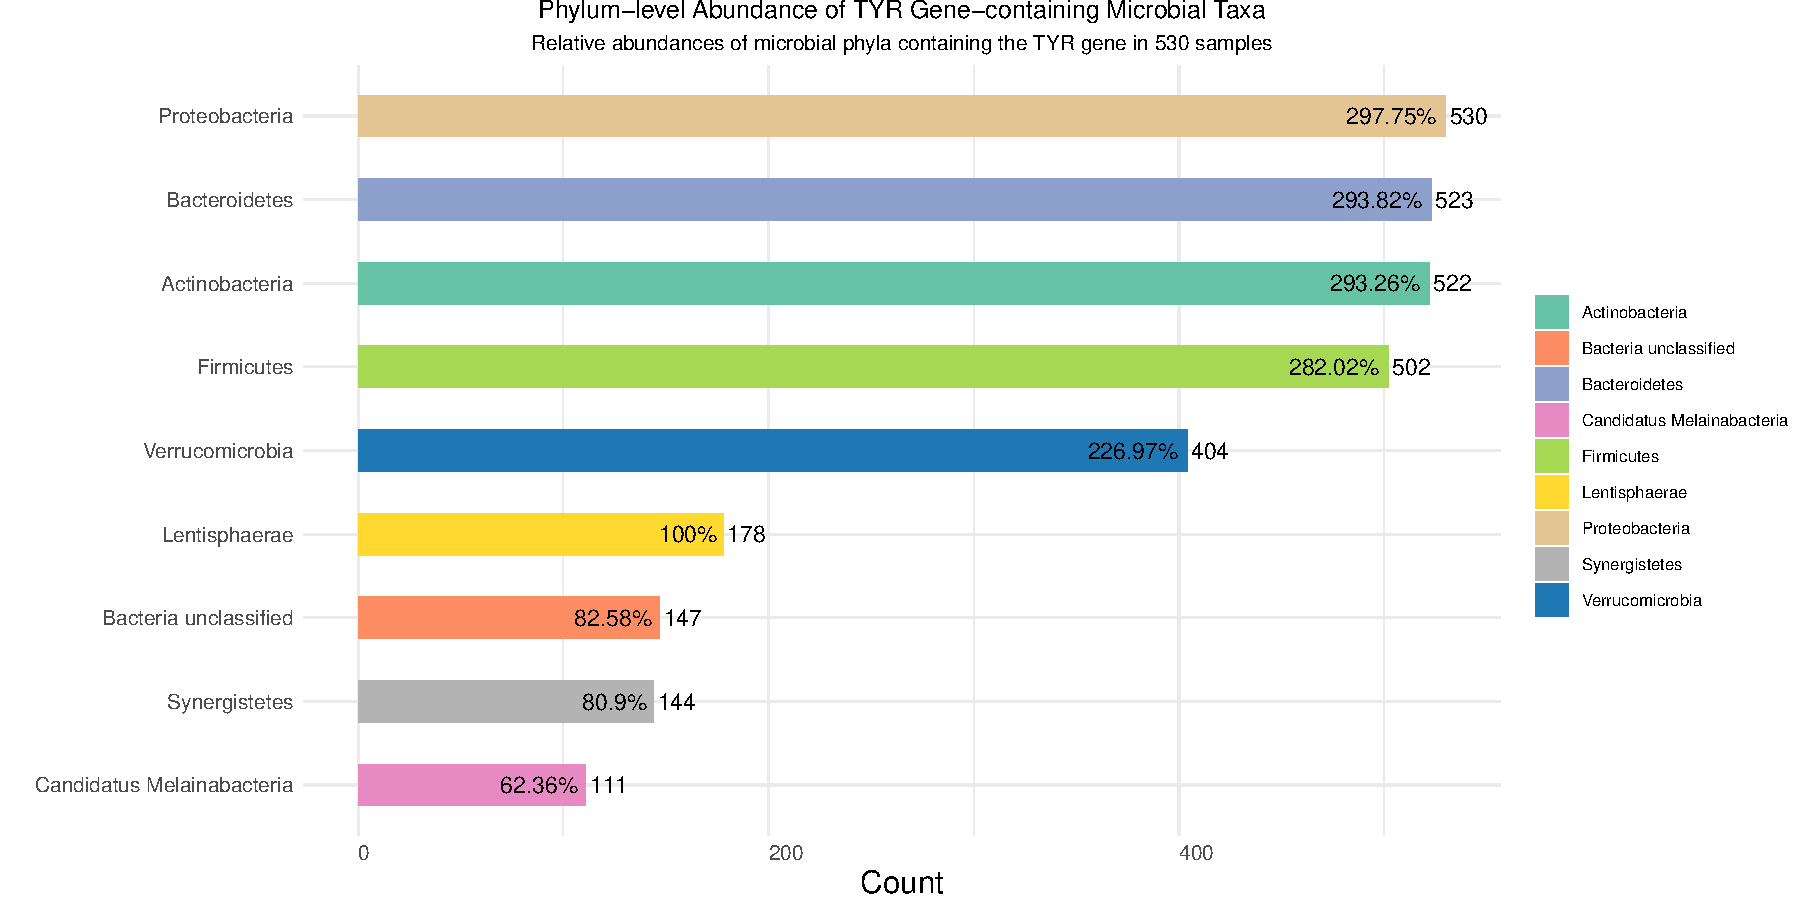
\includegraphics[width=1\linewidth]{pic/phylum.pdf} 
    \caption{\small\bfseries Phylum-level Bar Chart. Phylum-level bar chart depicting the relative abundances of microbial taxa containing the target gene TYR in 530 samples. Horizontal coordinates (X-axis): the count value of each microbial phylum in the sample or community. Vertical coordinate (Y-axis): different microbial phyla (Phylum). The number of clades was calculated as a percentage relative to the abundance of Lentisphaerae clades. Proteobacteria had the highest TYR enrichment. Candidatus Melainabacteria showed the lowest TYR enrichment.}
\end{figure}

The analysis provides insights into the diversity and relative abundance distribution of microbial phyla within TYR gene-containing microbial communities.Taking the phylum Lentisphaerae as the reference, percentage calculations were conducted for the remaining phyla. Four phyla, surpassing Lentisphaerae in abundance, demonstrated significant disparities at a categorical level. These results contribute valuable information for understanding the ecological characteristics and potential functional roles of microbial communities associated with the TYR gene, and offer valuable data for further investigations into microbial biodiversity and environmental microbiology.\\\\
Correlation analyses performed to investigate the relationship between bacterial population abundance and TYR gene abundance in the samples showed that scatter plots and best-fit straight lines showed a clear linear trend. This analysis is depicted in Figures 3 and 4, showing scatter plots and corresponding best-fit straight lines at the family and genus levels, respectively.\\\\
The slope of the best-fit straight line in the figure indicates the strength and direction of the linear association between the relative abundance of bacterial populations and TYR gene abundance. A positive slope suggests a positive correlation, indicating that as the relative abundance of bacterial populations increases, the TYR gene abundance also tends to increase. Conversely, a negative slope would indicate a negative correlation, implying that as the relative abundance of bacterial populations increases, the TYR gene abundance tends to decrease.

\begin{figure}[H]
    \centering
    \begin{minipage}{0.48\linewidth}
        \centering
        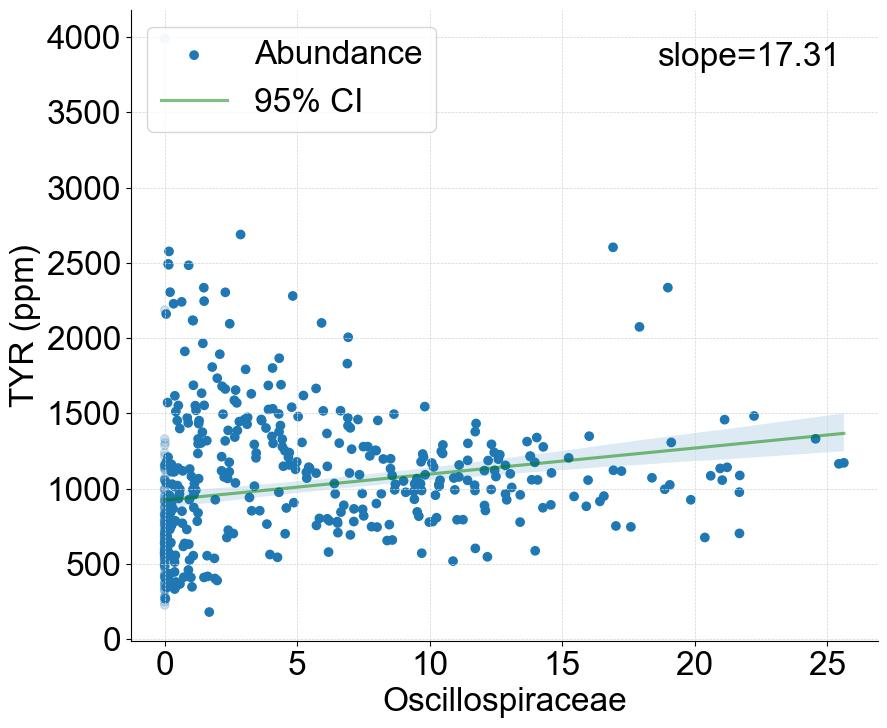
\includegraphics[width=\linewidth, height=0.8\linewidth]{pic/family/family1.jpg}
               \label{fig:image1}
    \end{minipage}
    \hfill
    \begin{minipage}{0.48\linewidth}
        \centering
        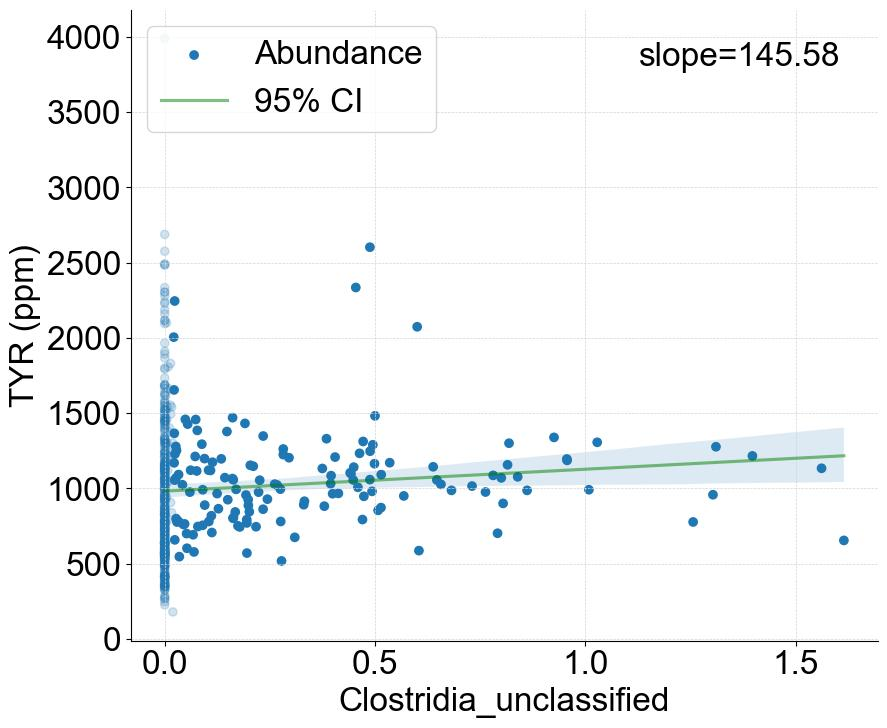
\includegraphics[width=\linewidth, height=0.8\linewidth]{pic/family/family2.jpg}
        \label{fig:fig:image2}
    \end{minipage}
    
    \vspace{1em} 
    
    \begin{minipage}{0.48\linewidth}
        \centering
        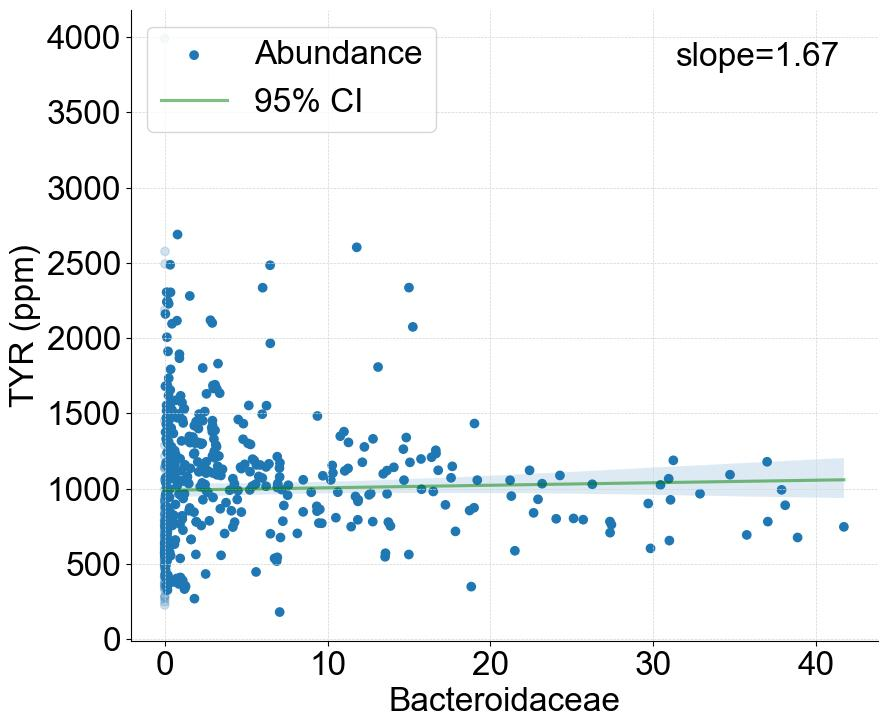
\includegraphics[width=\linewidth, height=0.8\linewidth]{pic/family/family3.jpg}
        \label{fig:image3}
    \end{minipage}
    \hfill
    \begin{minipage}{0.48\linewidth}
        \centering
        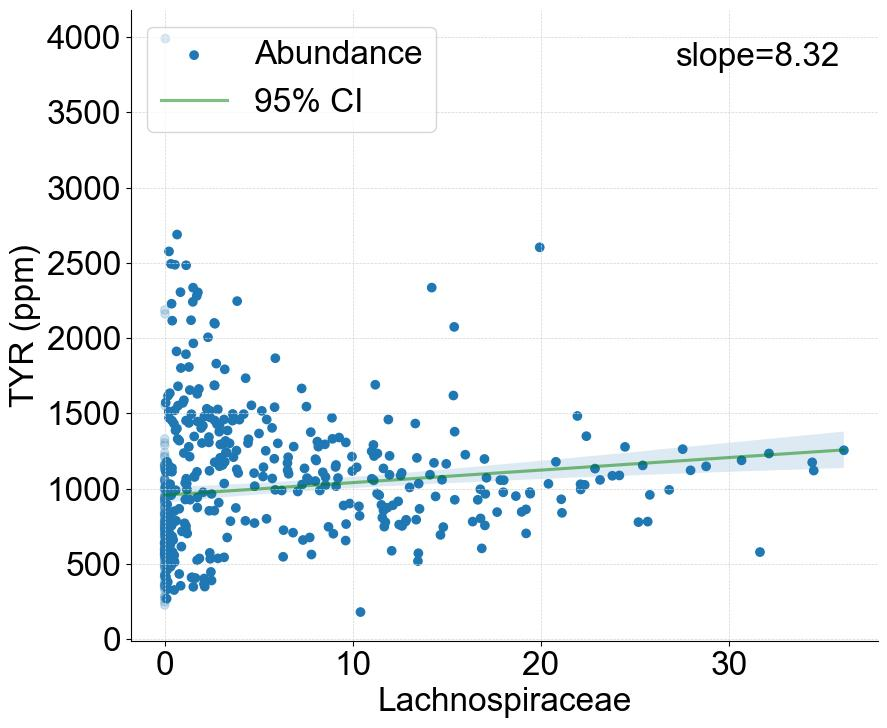
\includegraphics[width=\linewidth, height=0.8\linewidth]{pic/family/family4.jpg}
        \label{fig:image4}
    \end{minipage}

   \caption{\small\bfseries Linear regression relative population abundance and gene abundance based on Family. Only the 4 positive correlation scatter plots from the test data are shown.(Oscillospiraceae \& Clostridia\_unclassified \& Bacteroidaceae \& Bacteroidaceae}
\end{figure}
The presence of confidence bands in the figure is of great significance as well. These bands provide an estimation of the uncertainty associated with the predicted values and establish confidence intervals for the predicted values. The width of the confidence bands illustrates the range within which the predicted values are expected to fall with a certain level of confidence. This information aids in assessing the reliability and precision of the predictions made based on the correlation analysis. These plots provide a detailed visual representation of the correlations between bacterial population abundance and TYR gene abundance for various strains, supplementing the analysis conducted. The correlation coefficients of all fitted straight lines were recorded and ranked, and samples with slopes smaller or equal to less than 0 were specifically flagged and the weights were reduced by adjusting the parameters accordingly in the subsequent model building phase. Enrichment of samples with relative abundance less than 0.02 was observed in all scatter plots, with clustering occurring at a transparency of 80\%.

\begin{figure}[H]
    \centering
    \begin{minipage}{0.48\linewidth}
        \centering
        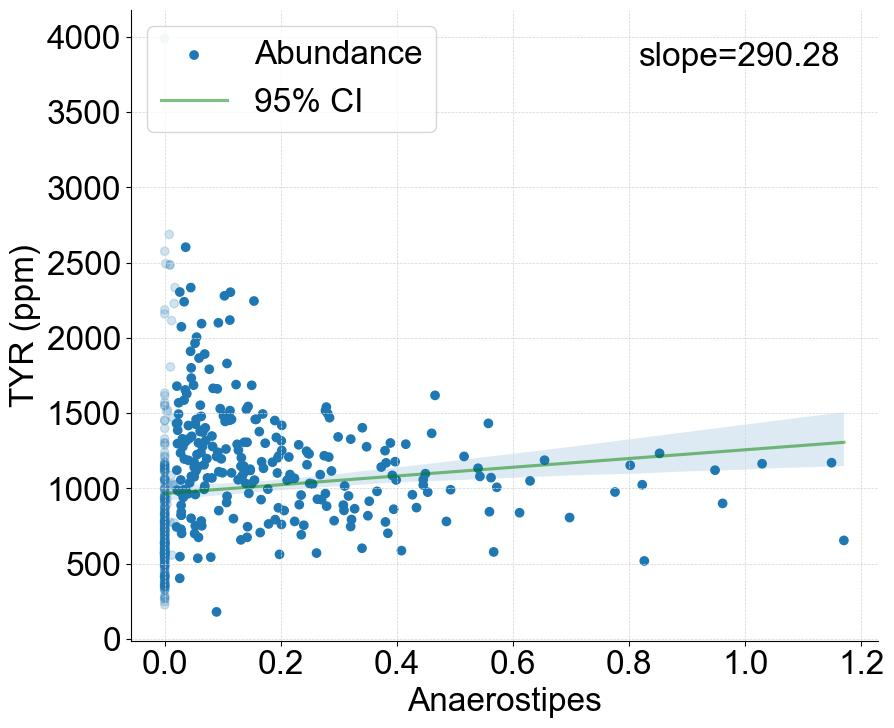
\includegraphics[width=\linewidth, height=0.8\linewidth]{pic/genus/genus1.jpg}
               \label{fig:image1}
    \end{minipage}
    \hfill
    \begin{minipage}{0.48\linewidth}
        \centering
        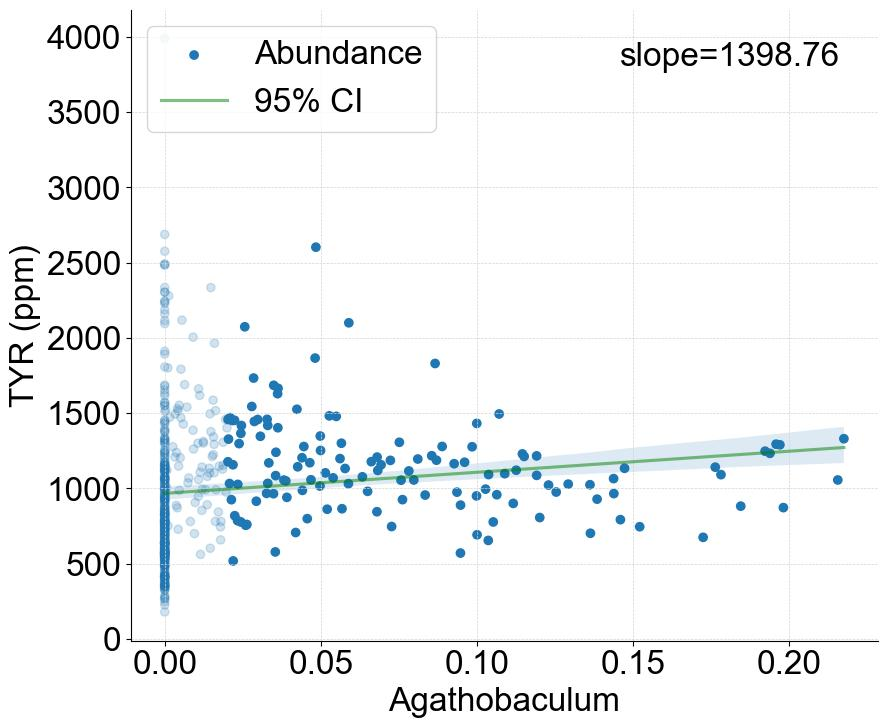
\includegraphics[width=\linewidth, height=0.8\linewidth]{pic/genus/genus2.jpg}
        \label{fig:fig:image2}
    \end{minipage}
    
    \vspace{1em} 
    
    \begin{minipage}{0.48\linewidth}
        \centering
        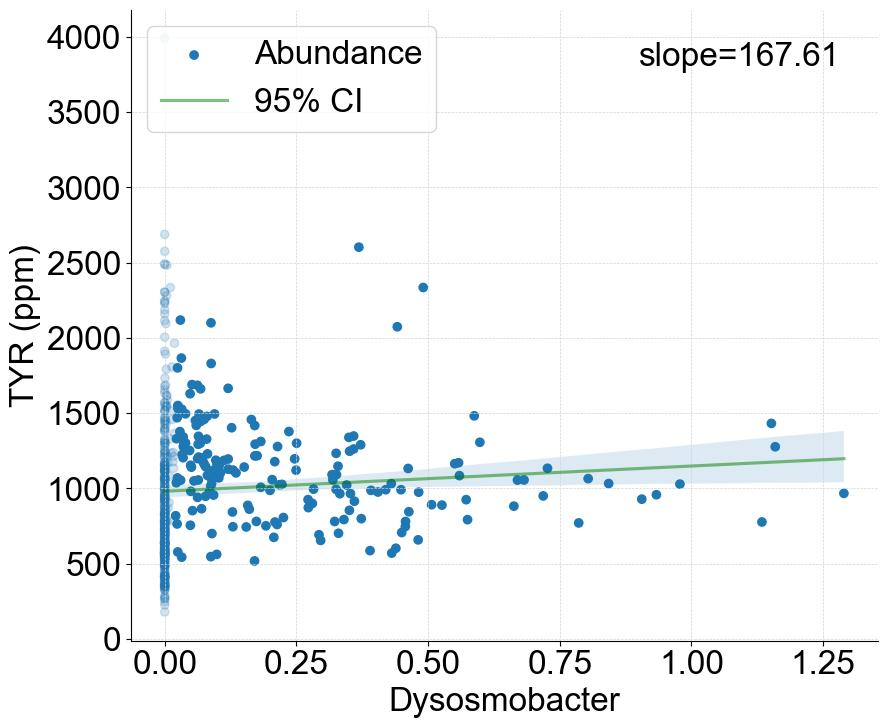
\includegraphics[width=\linewidth, height=0.8\linewidth]{pic/genus/genus3.jpg}
        \label{fig:image3}
    \end{minipage}
    \hfill
    \begin{minipage}{0.48\linewidth}
        \centering
        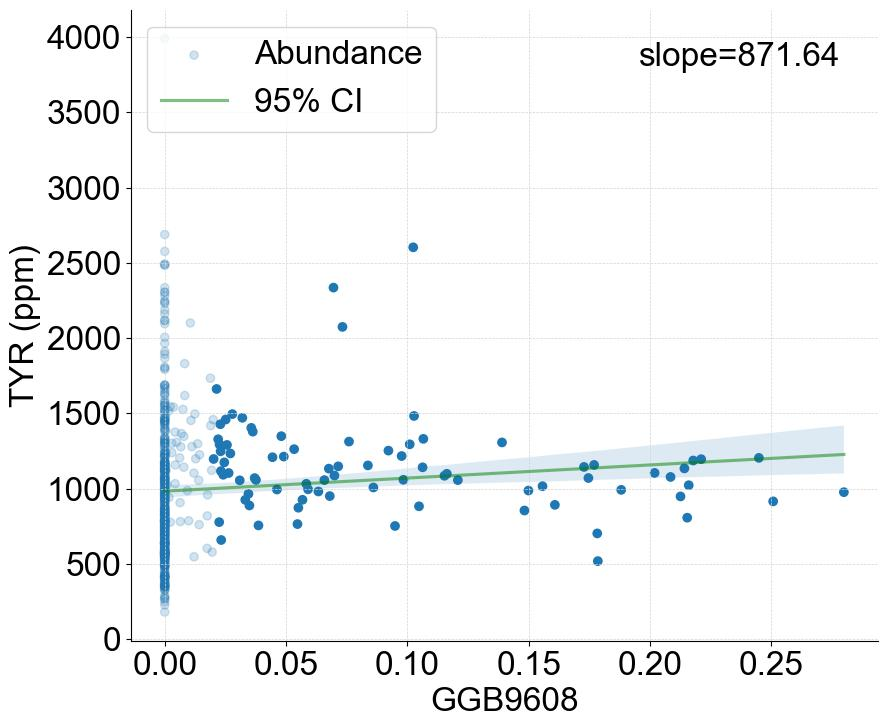
\includegraphics[width=\linewidth, height=0.8\linewidth]{pic/genus/genus4.jpg}
        \label{fig:image4}
    \end{minipage}

   \caption{\small\bfseries Linear regression relative population abundance and gene abundance based on Genus. The horizontal coordinate is the relative abundance of the population in the sample. The vertical coordinate is the abundance of the TYR gene in the sample.Transparency of points with relative abundance less than 0.02 will be increased to 80\%.Only the 4 positive correlation scatter plots from the test data are shown.(Anaerostipes \& Agathobaculum \& Dysosmobacter \& GGB9608}
\end{figure}
Figures 5\&6 show the results of model predictions based on both Family and Genus classes. The horizontal axis represents the test number ID of the random test subset, while the vertical axis represents the value of TYR gene abundance in the sample (PPM). The blue line corresponds to the actual observed values of the test dataset, while the red line represents the predicted values generated by the model for the same test dataset.\\\\
By visually comparing the blue and red lines, we can assess how well the model fits the test data. When the red line is closely aligned with the blue line, it indicates that the model's predictions are very close to the actual observations, suggesting that the model fits the test data well. Conversely, if there is a significant deviation between the red and blue lines, it indicates that the model's predictions deviate from the actual observations, suggesting that the model may not adequately account for changes in the test data.

\begin{figure}[H]
    \centering
    \begin{minipage}{1\linewidth}
        \centering
        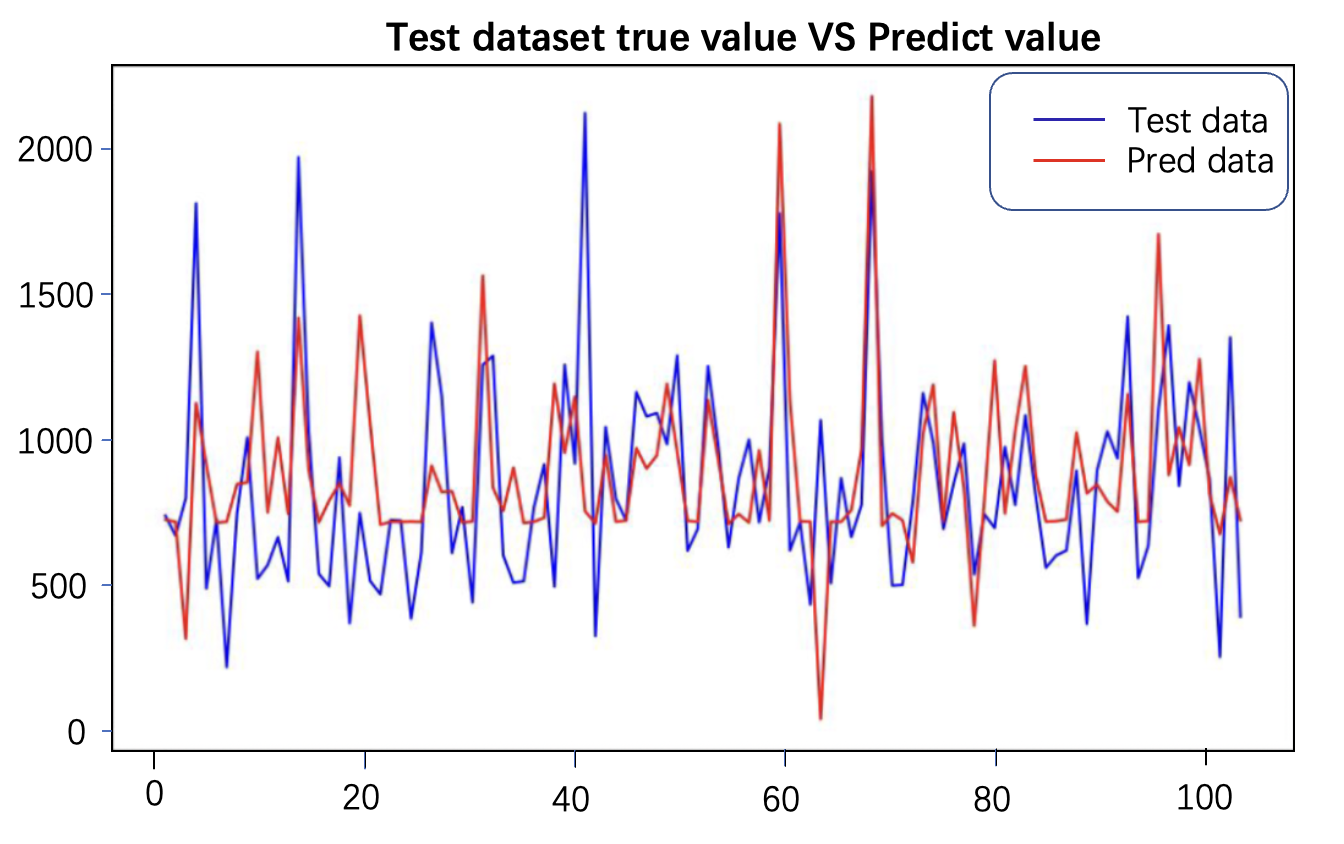
\includegraphics[width=\linewidth]{pic/family/pvst.png} 
         \caption{\small\bfseries Comparison of predicted abundance and observed values based on family level. The horizontal coordinate is the test set ID and the vertical coordinate is the predicted and actual value of TYR gene abundance.}
    \end{minipage}

    \vspace{0.1cm} % 
    \begin{minipage}{1\linewidth}
        \centering
        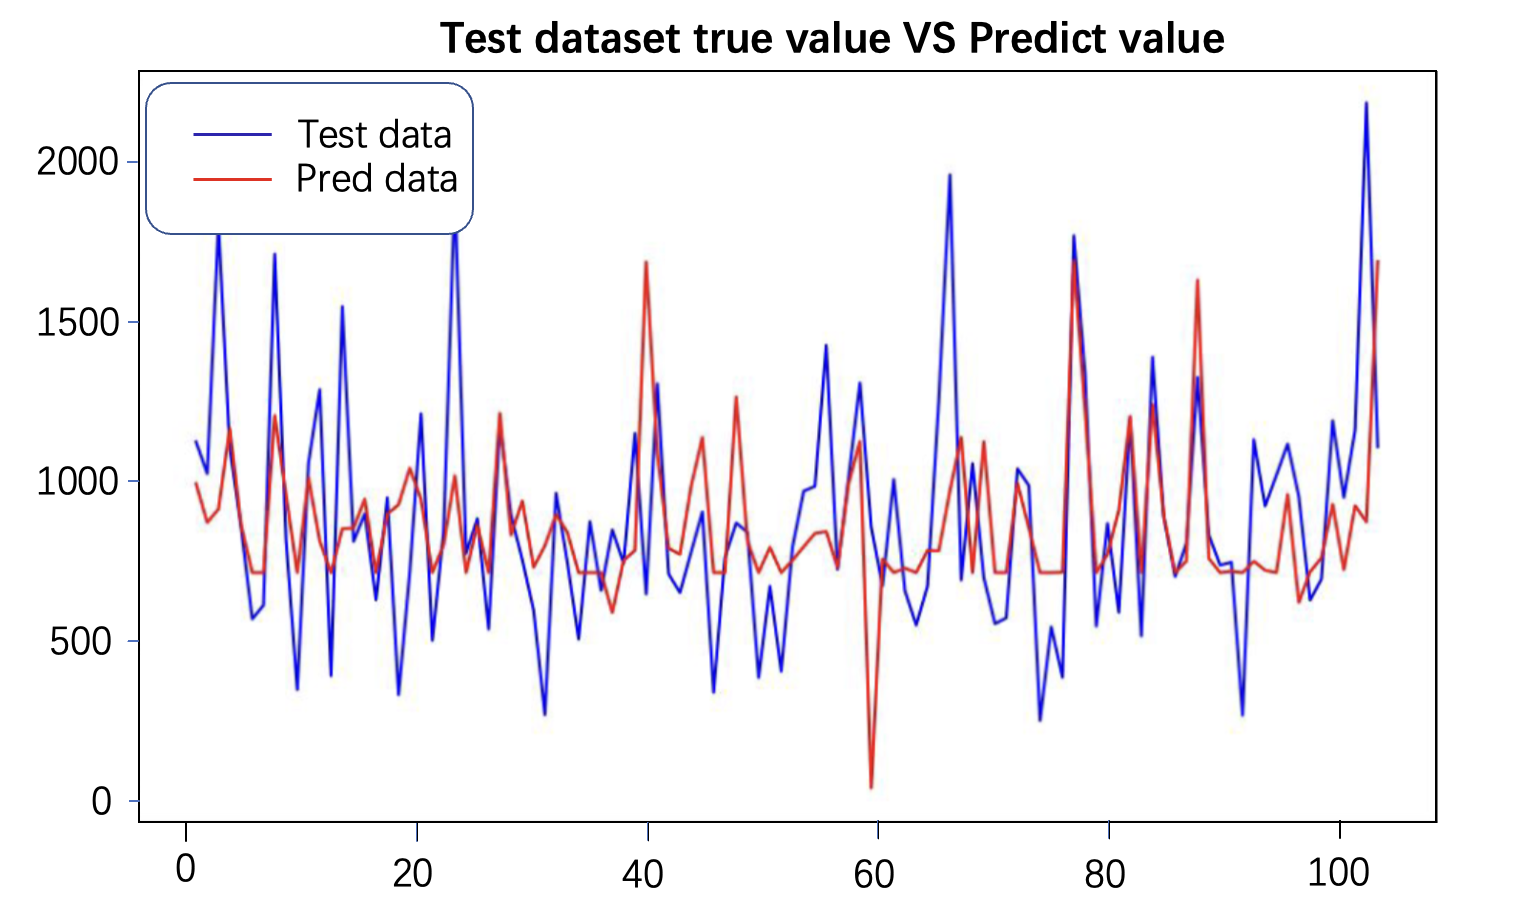
\includegraphics[width=\linewidth]{pic/genus/pvst.png} 
         \caption{\small\bfseries Comparison of predicted abundance and observed values based on genus level. The horizontal coordinate is the test set ID and the vertical coordinate is the predicted and actual value of TYR gene abundance.}
    \end{minipage}
    \label{fig:combined}
\end{figure}

In Figures 5 and 6, the red and blue lines for both levels (family and genus) show a significant overlap, indicating that the predictive model is capable of capturing the underlying relationship between bacterial population distribution and TYR gene abundance with a considerable degree of accuracy. The majority of the residuals fall within the range of plus or minus 500, suggesting that the predicted values closely align with the observed values for most of the samples. The average prediction error being at 25\% for an average abundance of 2000 ppm further proves the model's ability to accurately predict TYR gene abundance based on the bacterial population distribution.\\\\
The model's good fit to the test data indicates that the predictions are reliable and accurate for a substantial portion of the dataset. However, there are some interesting observations to be made from the data. The red line, which represents the predictions at the family level, exhibits a tendency to level off compared to the blue line (genus level). This indicates that there may be certain factors or complexities that the model fails to account for, particularly in extreme low peak sections.\\
The influence of the relative abundance of strains and the degree of TYR gene enrichment on model fitting becomes evident. Samples with higher relative abundance of strains show a relatively higher predictive fit, whereas lower relative abundance results in predicted data being biased high due to parameter corrections. This suggests that the model's performance may be influenced by the specific composition of bacterial strains in the test samples.\\\\
Moreover, the presence of outliers in the predicted data for certain test samples suggests the existence of unexplained sources of variation or factors not adequately addressed by the predictive model. These biases could arise from unmeasured variables, measurement errors, or other unknown factors that impact the relationship between bacterial population distribution and TYR gene abundance.
\begin{figure}[H]
    \centering
     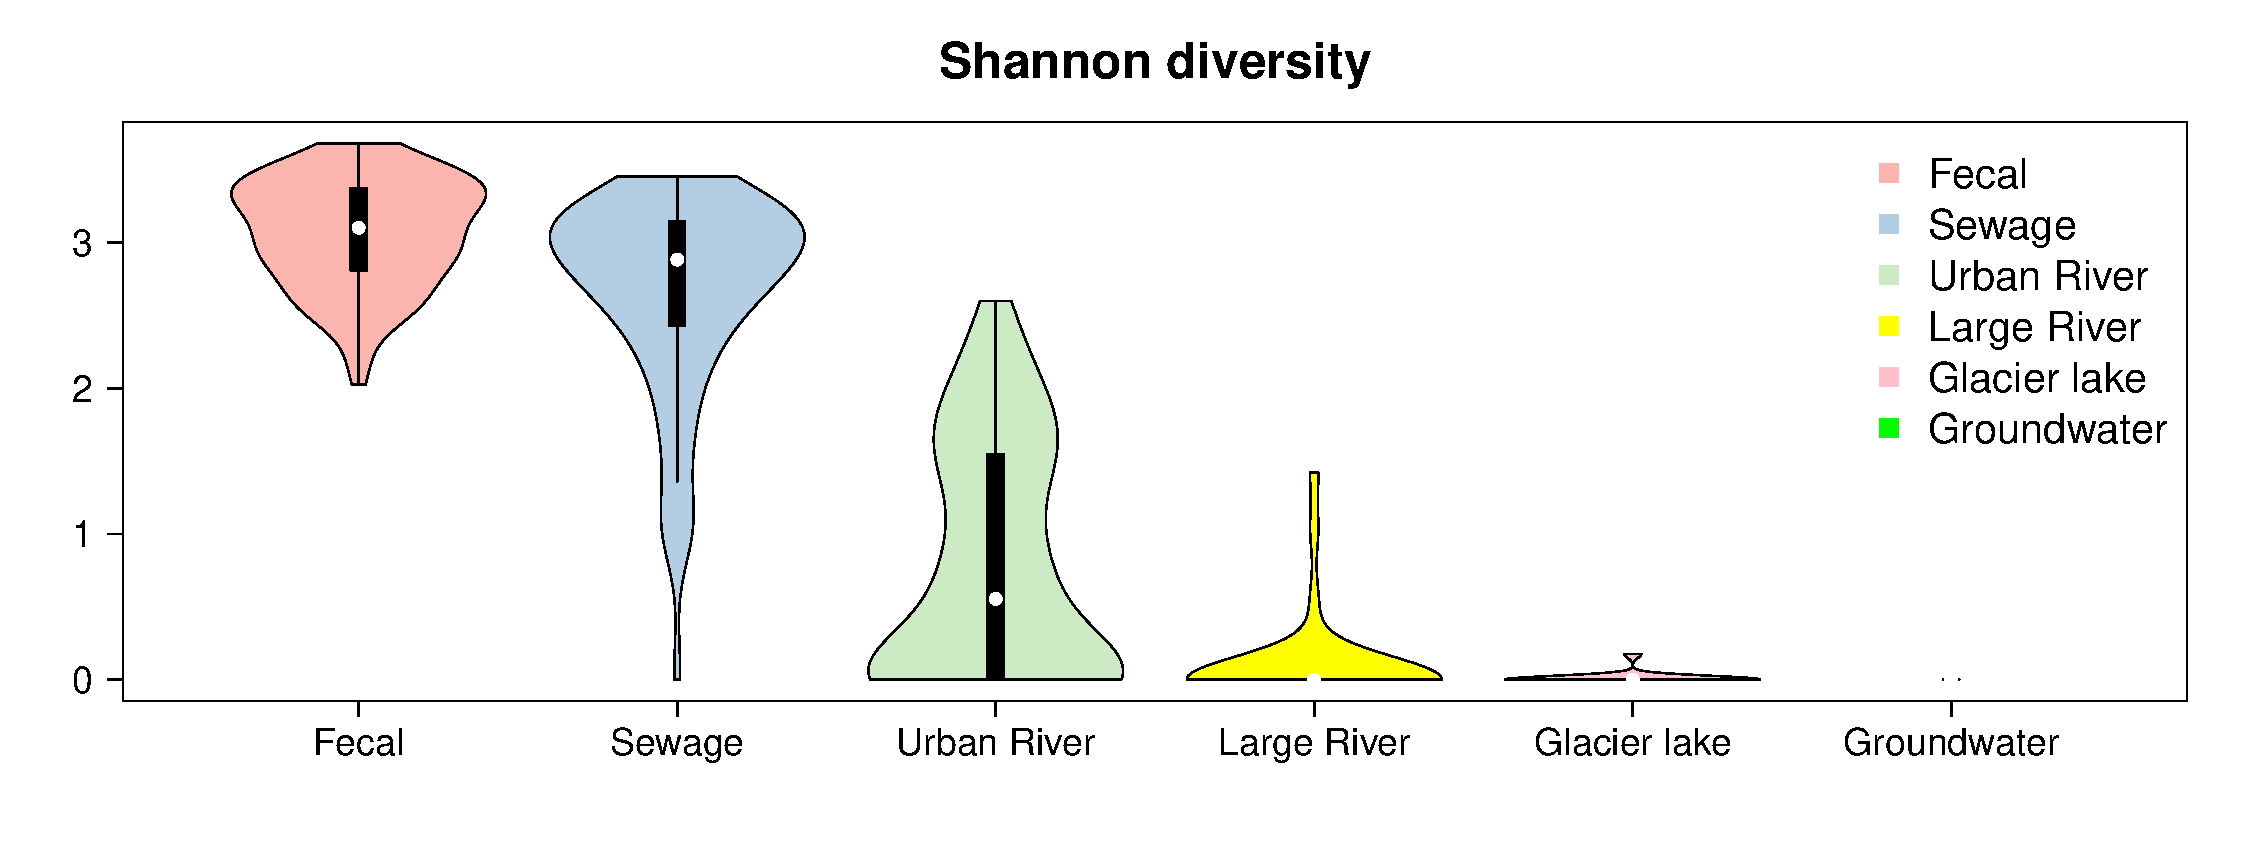
\includegraphics[width=1\linewidth]{pic/alpha.pdf} 
      \caption{\small\bfseries Alpha Diversity Plot. The horizontal coordinate is the sample category. The vertical coordinate is the shannon diversity value.}
\end{figure}
Figure 7 presents an alpha diversity plot based on the Shannon diversity index, revealing intriguing patterns of microbial diversity among bacterial hosts carrying the TYR gene across different environmental categories. The vertical axis represents the Shannon diversity value, reflecting the richness and evenness of species in each sample.\\\\
Notably, the Shannon diversity values are relatively high in feces and wastewater environments, approaching 3, indicating rich and evenly distributed microbial communities within TYR gene-carrying hosts. Conversely, the Shannon diversity value in urban river environments is moderate, around 0.5, suggesting lower species richness and uneven distribution of microbial taxa in hosts carrying the TYR gene. Meanwhile, the Shannon diversity values for the other three environmental categories are relatively low, around 0, indicating limited species diversity and uneven distribution of microbial taxa within TYR gene-carrying hosts.\\\\
Furthermore, the alpha diversity plots for each category exhibit non-square shapes and uneven distributions. Feces and wastewater environments are characterized by an inverted triangular pattern, highlighting the diversity and evenness of microbial communities within TYR gene-carrying hosts. In contrast, the plots for other environments show an upward triangular pattern, indicating lower species richness and less uniform distribution of microbial taxa in hosts carrying the TYR gene. This suggests significant differences in microbial community structure among different environments, and TYR gene-carrying microbial hosts in each environmental category possess unique compositions and ecological characteristics.
\begin{figure}[H]
    \centering
     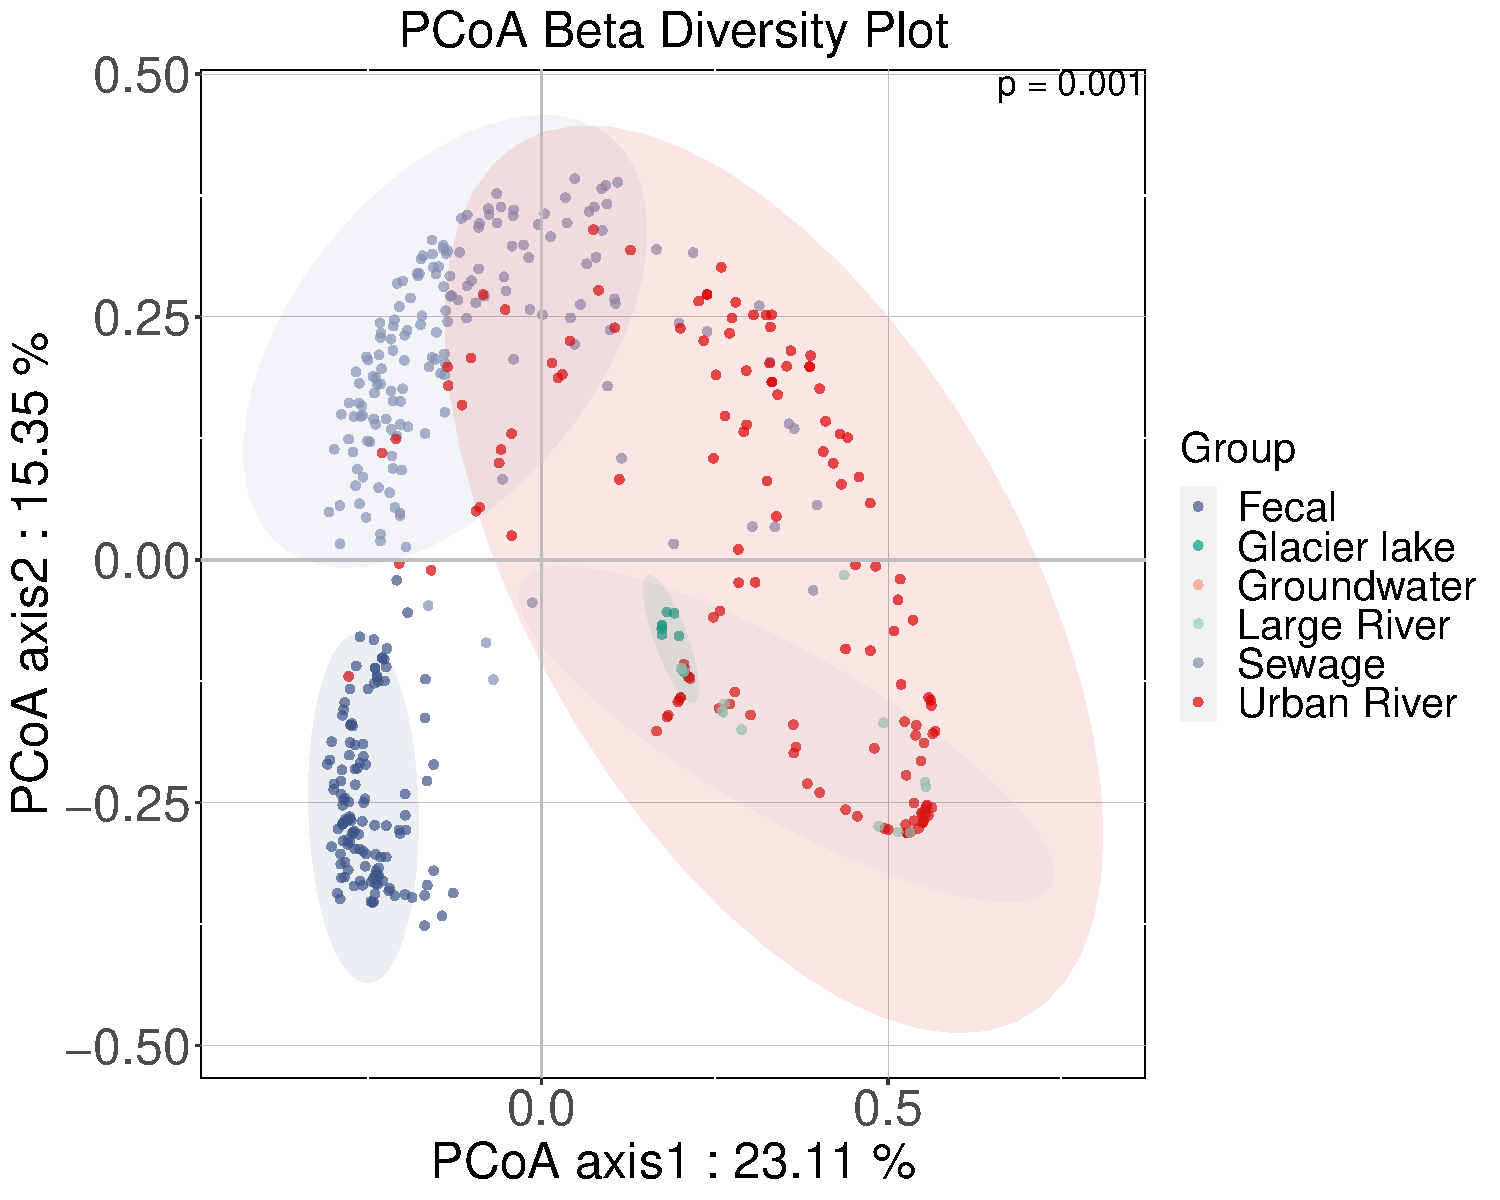
\includegraphics[width=1\linewidth]{pic/beta.pdf} 
      \caption{\small\bfseries Beta Diversity Plot. The horizontal and vertical coordinates represent the coordinate values of the samples on the different principal axes.}
\end{figure}
Figure 8 Beta diversity plots based on Bray-Curtis distances and visualised by principal coordinate analysis (PCoA) effectively reveal the overlapping patterns of TYR bacterial hosts in different environments, providing strong evidence of similarities and differences in bacterial community structure between samples. The ellipses in the plots represent confidence intervals that visualise the variability and dispersion of the sample groups in PCoA space. Samples within the same ellipse have similar bacterial community structures, while samples from different ellipses have more pronounced differences. Overlap of ellipses indicates partial similarity in bacterial composition, whereas non-overlap indicates significant differences between groups of samples.\\\\
Samples were significantly separated along the first principal axis (p=0.001), indicating significant overall differences in microbial composition across environments. This finding suggests that unique environmental conditions may create unique bacterial communities associated with TYR genes.\\\\
Notably, the figure shows that glacial lake, groundwater, and large river samples were completely included in the urban river clustering. This observation suggests a high degree of similarity in TYR bacterial hosts in these environments.\\\\
In addition, there was about 40\% overlap between the wastewater samples and the urban river samples, suggesting some similarity in their bacterial community structure. This commonality may be due to common anthropogenic influences or similar ecological factors. In contrast, fecal samples were significantly different from other environmental samples. This apparent difference highlights the unique microbial characteristics associated with faecal environments, which may be influenced by host-specific factors. In addition, due to the limited number of groundwater samples, only coordinate points were plotted and elliptical intervals were not calculated to ensure the accuracy of the analyses.\\\\
The overlapping patterns of TYR bacterial hosts in different environments were effectively demonstrated by PCoA's beta diversity plot based on Bray-Curtis distances, revealing similarities and differences in bacterial community structure. This analysis helps to understand how environmental conditions affect the microbial communities associated with TYR genes and provides important clues to the ecological significance of TYR gene-carrying bacterial hosts in different environments.\\\\
I conducted differential expression analysis to identify key predicted bacterial genera and performed Pearson correlation analysis with the TYR gene. The results of the correlation analysis are presented in Figure 9, displaying the strength of correlations between TYR gene abundance and bacterial taxa in six different sample environments. Among the 153 genera analyzed, 113 genera with significant correlations (correlation coefficient  \textgreater 0.2) were included in the visualization.\\\\
In Figure 9, each bacterial genus is represented as a node. The size of the node indicates the strength of the correlation between the genus and the TYR gene, with larger nodes indicating stronger correlations and smaller nodes indicating weaker correlations. The thickness of the lines connecting the nodes to the center represents the strength of the correlation, with thicker lines indicating stronger correlations and thinner lines indicating weaker correlations. The color of the lines is determined by the ranking of the correlation strength. The top 1.77\% of correlations are displayed in purple, representing two genera, Gemmiger and Escherichia, which have the strongest correlations with the TYR gene. The next 1.77-5.31\% of correlations are shown in red, encompassing six genera: Collisella, Streptococcus, Akkermansia, Bifidobacterium, Faecalibacterium, and an unidentified genus classified as \text{k\_\_Bacteria|p\_\_Firmicutes|c\_\_CFGB10477|o\_\_OFGB10477|f\_\_FGB10477|g\_\_GGB9345}. Fourteen genera with correlations ranging from 5.31\% to 12.39\% are represented by orange lines. The remaining genera with weaker correlations are shown with light orange lines at 40\% transparency.\\\\
These significant correlations indicate that these bacterial taxa may play crucial roles in the regulation and function of the TYR gene in different sample environments. The visualization of these correlations in Figure 9 provides valuable insights into the potential interactions between microbial communities and the TYR gene, contributing to a better understanding of the ecological and functional implications of the TYR gene in diverse environments.
\begin{figure}[H]
    \centering
    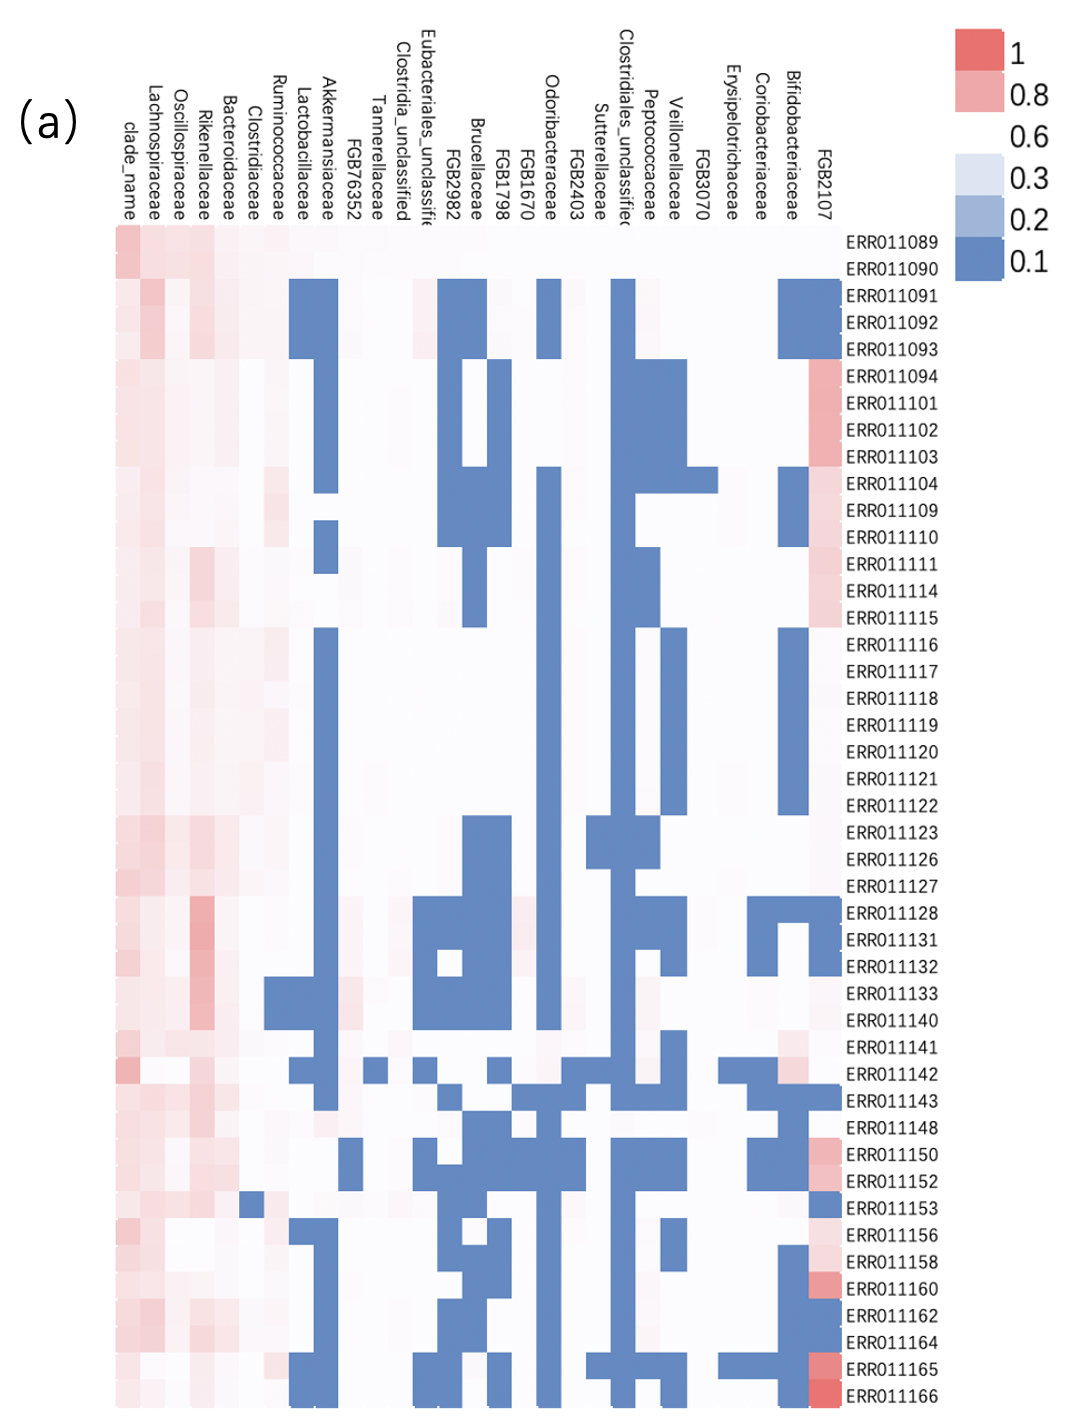
\includegraphics[width=1\linewidth]{pic/heatingmapfamily.png}
\end{figure}
\newpage
\begin{figure}[H]
    \centering
    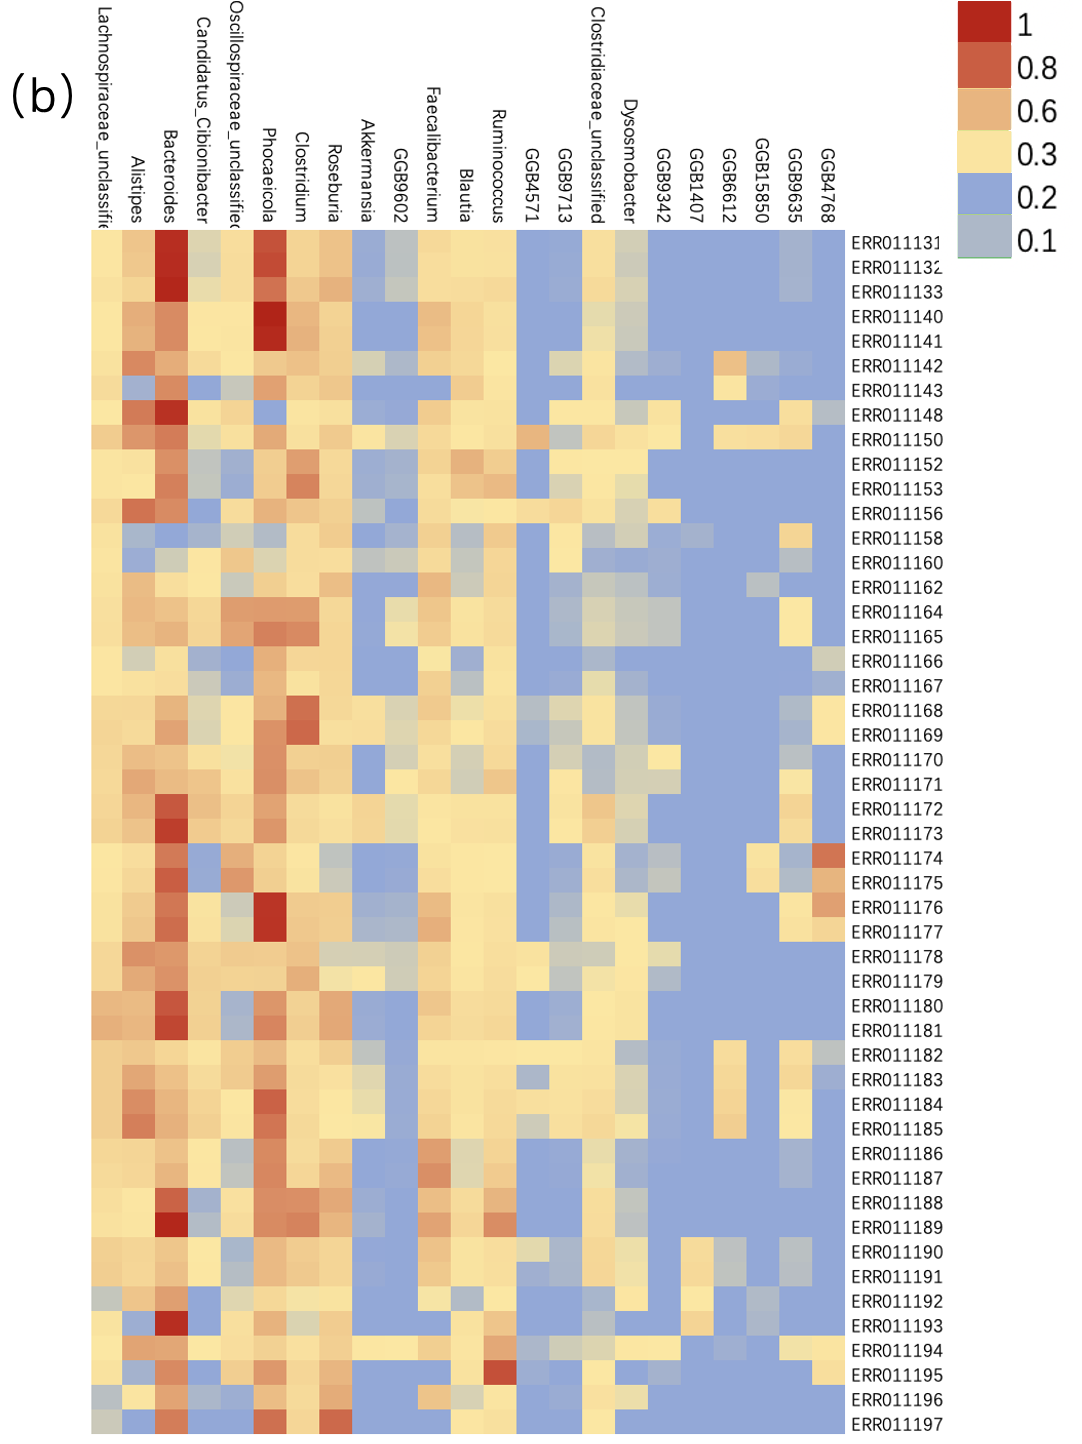
\includegraphics[width=1\linewidth]{pic/heatingmapgenus.png}
\end{figure}
\begin{figure}[H]
    \centering
     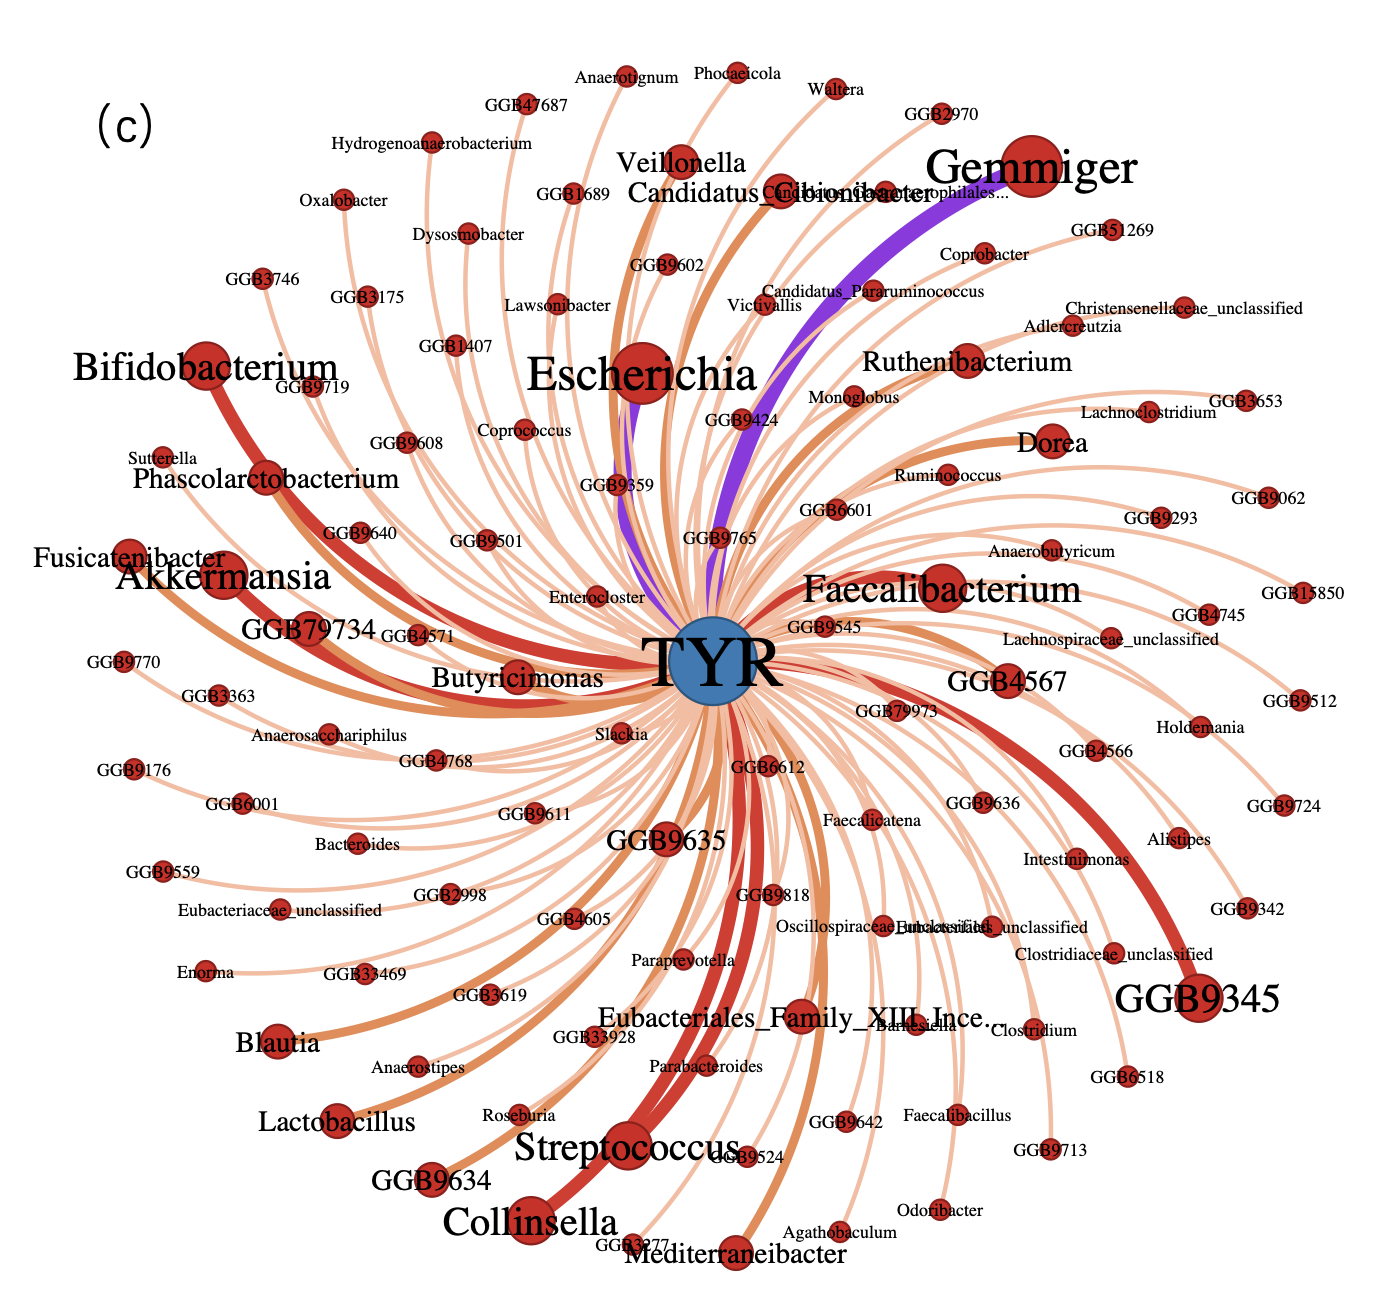
\includegraphics[width=1\linewidth]{pic/connection.png} 
     \caption{\small\bfseries (a) Schematic of TYR gene heat based on FAMILY level. The first 44 numbered IDs and 28 strains are shown. (b) Schematic of TYR gene heat based on genus level. The first 49 numbered IDs and 23 strains are shown. (c)Network plot of association of significantly related species with TYR genes. The thickness of the connecting line between the node and the centre and the size of the node represent the strength of the correlation. The colour shade of the connecting line indicates the order of significance of the correlation between the node and the central TYR gene.}
\end{figure}

\section{Discussion}

In this study, I aimed to bridge the knowledge gap in identifying bacterial hosts of the TYR gene in different environments by applying a robust machine learning framework. I utilized multivariate linear regression modeling to predict the abundance of TYR genes based on the analysis of bacterial community abundance data obtained from Metagenomic studies. Our findings demonstrate the great potential of using machine learning techniques to effectively identify potential bacterial hosts responsible for TYR activity in the environment.\\\\
My findings demonstrate that (1) the abundance and hosts of the TYR gene in microbial communities can be predicted using machine learning techniques and to a certain extent can be useful for subsequent targeted identification of incompletely recognised strains (2) the abundance of the TYR gene in microbial hosts in different environments is comparable to that of Gemmiger, Escherichia, Collisella, Streptococcus, Akkermansia, Bifidobacterium, Faecalibacterium and the not fully recognised \text{k\_\_Bacteria|p\_\_Firmicutes|c\_\_CF}\\
\text{GB10477|o\_\_OFGB10477|f\_\_FGB10477|g\_\_GGB9345} bacteria are extremely correlated (3) The diversity of microbial hosts carrying TYR genes in different environments reflects the variability. Fecal and wastewater environments had abundant and evenly distributed host communities. Urban rivers were not particularly characterised in terms of colony numbers and diversity. Groundwater and glacial lake environments still need further study.\\\\
I successfully developed a multivariate linear regression model using the relative abundance matrix of bacterial colonies and the gene abundance matrix to predict TYR gene abundance. The model's good fit to the test data indicates that the predictions are reliable and accurate for a substantial portion of the dataset. However, I observed some outliers in the predicted data, suggesting the existence of unexplained sources of variation or factors not adequately addressed by the predictive model. Further research is needed to identify and account for these factors to improve the model's performance.Even so, my current research continues to demonstrate that it is feasible to use machine learning techniques to help predict the abundance and hosts of TYR genes in microbial communities. To a certain extent, expensive upfront full molecular diagnostic identifications can be circumvented \citep{varadi2017methods}, opening up new possibilities for subsequent purification and identification of bacteria.\\\\
The correlation analysis between TYR gene abundance and bacterial taxa provided valuable insights into the potential interactions between microbial communities and the TYR gene in different environments. Among the 153 genera analyzed, 113 genera showed significant correlations with the TYR gene, indicating their potential roles in the regulation and function of the TYR gene. This information helps to better understand the ecological and functional implications of the TYR gene in diverse environments.\\\\
The alpha diversity and beta diversity analysis revealed intriguing patterns of microbial diversity among bacterial hosts carrying the TYR gene across different environmental categories \citep{socolar2016should}. Feces and wastewater environments exhibited high Shannon diversity values, indicating rich and evenly distributed microbial communities within TYR gene-carrying hosts \citep{thukral2017review}. On the other hand, urban river environments showed moderate Shannon diversity values, suggesting lower species richness and uneven distribution of microbial taxa in hosts carrying the TYR gene. These findings emphasize the differences in microbial community structure among different environments and the unique compositions and ecological characteristics of TYR gene-carrying microbial hosts in each category.\\\\
The association network diagram constructed using significant correlations between TYR gene abundance and bacterial taxa provided a visual representation of the relationships between TYR genes and specific strains. The strength and direction of the correlations were represented by the size and thickness of the nodes and connecting lines, respectively. This network diagram helps to identify key predicted bacterial genera that are significantly associated with the TYR gene and contributes to a better understanding of the potential microbial hosts responsible for TYR activity.In particular, the incompletely identified bacterium \text{k\_\_Bacteria|p\_\_Firmicutes|c\_\_CFGB10477|o\_\_OFGB10477|f\_\_FGB10477}\\
\text{|g\_\_GGB9345} was successfully identified. This suggests that the use of a sufficiently rich metagenome can circumvent to some extent the time cost required for experimental validation of identifications, and improve the efficiency and accuracy of identifications by predictively probing high-probability strains obtained by screening.\\\\
Overall, my research has provided valuable information to the field of environmental microbiology and carbon cycle research. Using machine learning techniques, I have made significant progress in identifying potential bacterial hosts of TYR genes in sampled environments, and through machine learning algorithms, I have calculated enriched strains of TYR genes and possible hosts for subsequent qualitative validation. This in part contributes to the subsequent understanding of the complex dynamics of TYR in the global carbon cycle and environmental processes. Identifying as many TYR hosts as possible can greatly assist in subsequent conditional and quantitative studies of the role of TYR.\\\\
However, there are certain limitations to my research. The dataset used for model training and validation was based on publicly available Metagenomic datasets that may not fully represent the diversity of bacterial communities in all environments. Future studies should consider using larger and more comprehensive datasets to improve the accuracy and generalisation of predictive models. In addition, further experiments are needed to validate the predictive correlation between bacterial taxa and TYR gene abundance. Moreover, the model in this study discarded many influencing factors and variables in the real environment. For example, sampling time, sampling temperature, sample size, geographic location elevation and many other scientific factors. Subsequently, the model can be optimised by adding subject variables as needed, or changing variables to target variables for specific identification based on this algorithm.\\\\

\section{Conclusions}
In summary, my study takes the perspective of the importance of bacteria in ecosystems in reducing greenhouse gas emissions and mitigating climate change, using the application of multiple linear regression and machine learning techniques in order to be able to identify potential bacterial hosts of TYR genes in different environments. This provides valuable assistance for future studies on the ecological and functional significance of TYR in different environments. It lays the foundation for future studies on microbial diversity of ecosystems, environmental microbiology and carbon cycle processes.
 
\newpage    
\bibliographystyle{apalike}
    \bibliography{projectref}
\end{document}